\section{In-hand Manipulation Experiments}
\label{sec:exp}

\begin{figure}
\centering
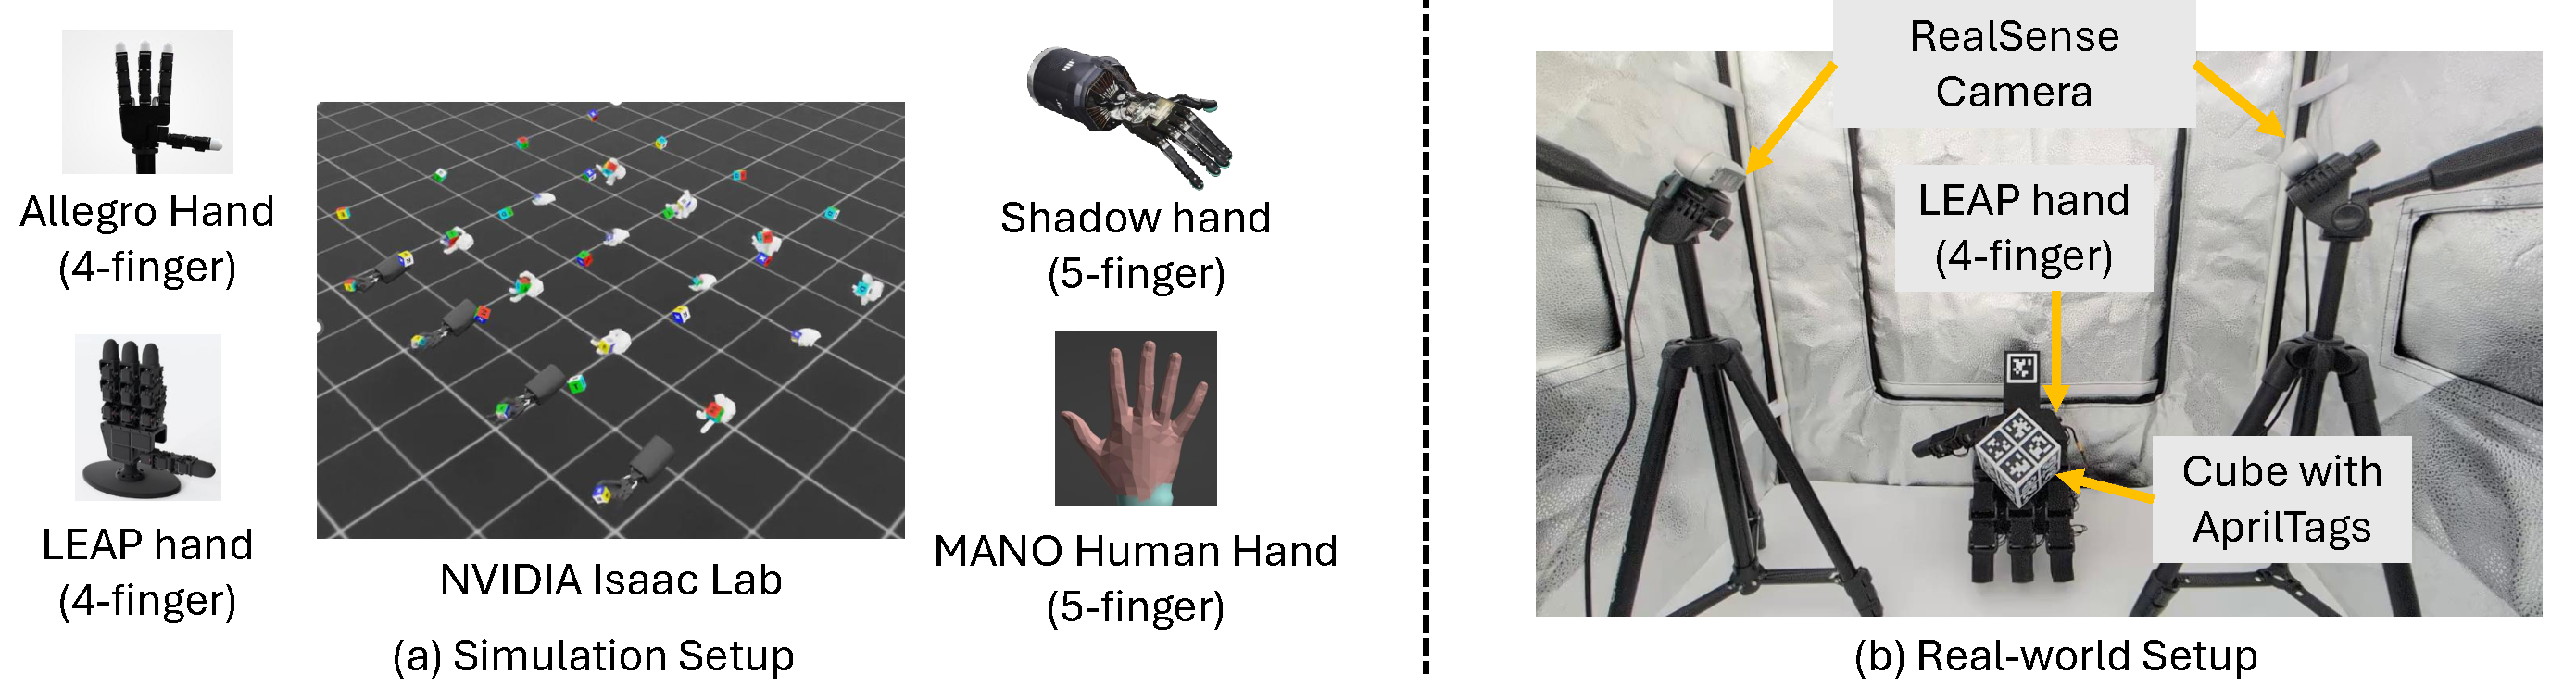
\includegraphics[width=\linewidth]{figures/tasks.pdf}
\vspace{-3mm}
\caption{(a) Simulation setup with 4 hands (b) Our real-world setup of the LEAP hand}
\label{fig:real_world_setup}
\vspace{-4mm}
\end{figure}

\subsection{Experimental Setup}

\paragraph{Tasks.}
We evaluate our method on the task of in-hand cube reorientation in both simulation and the real world. i) For simulation, We use the Repose Cube simulation in NVIDIA Isaac Lab~\cite{mittal2025isaaclab}, and adapt it to use our sphere controller for four hands: Leap Hand~\cite{shaw2023leaphand} and Allegro Hand~\cite{allegrohand} (4 fingers each), and Shadow Hand~\cite{shadowhand} and a simulated MANO human hand model~\cite{MANO:SIGGRAPHASIA:2017} (5 fingers each) as shown in Fig.~\ref{fig:real_world_setup}(a). In each episode in simulation, the robotic hand is required to sequentially reach 10 target cube orientations. If the cube falls, the environment is reset and the remaining reorientation attempts continue until all 10 targets have been evaluated.  ii) In the real world, we conduct experiments with a LEAP hand as shown in Fig.~\ref{fig:real_world_setup}(b). For each trial in the real world, we run the policy until the cube falls. In both simulation and real-world experiments, each target orientation must be reached within 30 seconds. Otherwise, the attempt is considered a failure.


\vspace{-2mm}
\paragraph{Evaluation Metrics.}
We report two primary evaluation metrics. The \textbf{Average Consecutive Reorientations} measures the average number of consecutive successful reorientations achieved before the first cube drop, with a maximum value of 10 in our simulation environment. The \textbf{Success Rate} measures the percentage of successful individual reorientation attempts, where a trial is considered successful if the cube reaches the target orientation without falling. All simulation results are evaluated using 1000 parallel environments. As a baseline, we compare against a policy trained to directly predict hand joint positions while using joint positions and velocities as the input state.



% \begin{figure}[h]
% \centering
% \includegraphics[width=0.25\linewidth]{example-image}
% \caption{Homogeneous observations across Grippers.}
% \label{fig:Homogeneous observations}
% \end{figure}

% \paragraph{Manipulation Policies.}
% We train the in-hand manipulation policies using the RSL-RL implementation of PPO~\cite{schwarke2025rslrl} with a lightweight actor-critic network. The policy outputs actions in the form of sphere deformations, where each finger's lateral movement is controlled by one driving plane with two driving vectors. \yu{Briefly mention how to deal with both 4 and 5 fingers? So we can use the same action for all hands.} These vectors directly influence the encompassing joints through the CIK algorithm. We adopt the same reward formulation as the original Isaac Lab~\cite{mittal2025isaaclab} environment and use identical reward settings for all models and baselines to ensure fair comparisons. For observations, we use homogeneous observations expressed in the canonical sphere coordinate frame and normalized by the corresponding hand-specific sphere radius. This is necessary because raw joint observations are incompatible across robotic hands with different kinematic structures and numbers of fingers. Additional training and observation details are provided in the Appendix~\ref{appendix:training}.

\vspace{-2mm}
\paragraph{Manipulation Policies.}
We train in-hand manipulation policies using the RSL-RL implementation of PPO~\cite{schwarke2025rslrl} with a lightweight actor-critic network. The policy outputs sphere deformations, where each finger is controlled by one driving plane with two driving vectors. To support both 4-finger and 5-finger hands within a unified action space, we add an extra driving plane at the ring-finger position for 4-finger embodiments. We adopt the same reward formulation as the original Isaac Lab~\cite{mittal2025isaaclab} environment and use identical reward settings for all models and baselines. For observations, we use homogeneous observations expressed in the canonical sphere coordinate frame and normalized by the corresponding hand-specific sphere radius, enabling a shared observation space across robotic hands with different kinematic structures and numbers of fingers. Together with the unified action representation, \emph{this allows a single policy to operate across all robotic hands used in our experiments.} Additional training details are provided in Appendix~\ref{appendix:training}.


% Each finger is discretized into seven equidistant points along its length, from which we retain only the center and fingertip positions (duplicating the ring-finger observations for four-finger hands to maintain dimensional consistency). The observation vector additionally contains the goal rotation, object pose, linear and angular velocities, the quaternion difference to the target orientation, fingerprint point positions and velocities, and the policy’s previous actions. 


% \yu{Talk about state, action, and reward of the policy here.}



% \begin{table}[h!]
%     \centering
%     \caption{Sphere Controller for In-hand Cube Reposing. Results are reported as (Success Rate / Average Consecutive Reposes).}
%     \label{tab:sphere_controller}
%     \begin{tabular}{lccc}
%         \toprule
%         \textbf{Training Hands} & \textbf{Testing Hands} & \textbf{Controller} & \textbf{Metrics} \\
%         \midrule
%         Allegro     & Allegro   & Sphere  & 99.21 / 9.55 \\

%         Allegro      & Allegro  & Joint  & 97.44 / 8.45 \\         

%         Allegro + LEAP + Shadow + MANO      & Allegro  & Sphere  & 99.00 / 9.42 \\

%         LEAP + Shadow + MANO      & Allegro (zero-shot)  & Sphere  & 97.26 / 8.52 \\

%         \hline
        
%         LEAP        &  LEAP  & Sphere  & 99.81 / 9.85 \\


        
%         LEAP        &  LEAP  & Joint  & 98.65 / 9.23 \\
        
%         Allegro + LEAP + Shadow + MANO         &  LEAP  & Sphere  & 98.95 / 9.50 \\

%         Allegro + Shadow + MANO         &  LEAP (zero-shot)  & Sphere  & 92.81 / 6.85 \\ 

%         \hline

%         Shadow & Shadow & Sphere & 99.52 / 9.69 \\

%         Shadow & Shadow & Joint & 97.75/ 8.85 \\

%         Allegro + LEAP + Shadow + MANO         &  Shadow  & Sphere  & 98.50 / 9.09 \\

%         Allegro + LEAP + MANO         &  Shadow (zero-shot)  & Sphere  & 81.88 / 4.00 \\

%         \hline

%         MANO & MANO & Sphere & 99.76 / 9.86 \\

%         MANO & MANO & Joint & 99.67 / 9.74 \\

%         Allegro + LEAP + Shadow + MANO         &  MANO  & Sphere  & 99.33 / 9.57 \\

%         Allegro + LEAP + Shadow         &  MANO (zero-shot)  & Sphere  & 98.72 / 9.41 \\        
        
%         \bottomrule
%     \end{tabular}
% \end{table}






\subsection{Simulation Results}


\begin{table}[h]
\centering
\caption{
In-hand cube reorientation results. Metrics are reported as (Success Rate / Average Consecutive Reorientations). 
\textbf{Single-Hand}: trained only on the target hand.
\textbf{Joint Control}: baseline joint-space controller trained on the target hand.
\textbf{Multi-Hand}: trained on all four hands.
\textbf{Zero-shot}: trained on all hands except the target hand.
}
\label{tab:main_results}

\setlength{\tabcolsep}{4pt}
\scalebox{0.8}{
\begin{tabular}{lcccc}
\toprule
\textbf{Test Hand} & \textbf{Single-Hand} & \textbf{Joint Control} & \textbf{Multi-Hand} & \textbf{Zero-shot} \\
\midrule
Allegro 
& \textbf{99.1 / 9.6 $\pm$ 1.7} 
& 98.5 / 9.2 $\pm$ 2.2
& 99.2 / 9.5 $\pm$ 1.9
& 95.3 / 7.7 $\pm$ 3.4\\

LEAP 
& \textbf{99.7 / 9.8 $\pm$ 1.1} 
& 98.6 / 9.3 $\pm$ 1.2
& 99.1 / 9.5 $\pm$ 1.9
& 95.5 / 7.7 $\pm$ 3.5 \\

Shadow 
& \textbf{99.3 / 9.6 $\pm$ 1.6} 
& 98.0 / 9.1 $\pm$ 1.9
& 98.7 / 9.2 $\pm$ 2.3
& 85.7 / 4.4 $\pm$ 3.7\\

MANO 
& \textbf{99.8 / 9.9 $\pm$ 1.0} 
& 99.6 / 9.8 $\pm$ 1.4
& 99.5 / 9.8 $\pm$ 1.2
& 98.1 / 8.9 $\pm$ 2.6\\

\bottomrule
\end{tabular}
}
\vspace{-2mm}
\end{table}

\paragraph{Main Results.}
Table~\ref{tab:main_results} evaluates the proposed sphere controller across four robotic hands on the in-hand cube reorientation task. We compare four training settings: \emph{Single-Hand}, where a separate policy is trained for each hand individually; \emph{Joint Control}, a baseline controller operating directly in joint space; \emph{Multi-Hand}, where a single policy is jointly trained across all hands using the proposed UHAS representation; and \emph{Zero-shot}, where the target hand is excluded during training and evaluated without finetuning.

The proposed UHAS representation achieves consistently strong performance across all hands and generally outperforms the joint-space baseline in both task success and long-horizon stability. Importantly, the Multi-Hand results show that a single shared policy can achieve performance comparable to embodiment-specific policies, while the Zero-shot results demonstrate meaningful transfer to previously unseen robotic hands despite substantial differences in kinematic structure and finger morphology. These results highlight the effectiveness of the proposed UHAS representation for cross-embodiment dexterous manipulation.

\vspace{-2mm}
\paragraph{Cross-Morphology Generalization.}
Table~\ref{tab:finger_generalization} evaluates transfer across robotic hands with different numbers of fingers. We train one policy on the two 5-finger hands (MANO and Shadow) and another on the two 4-finger hands (Allegro and LEAP), then evaluate both policies on all four hands. During deployment, models are applied directly without additional processing, where 5-finger models use one driving plane with its vectors per finger, while 4-finger models duplicate the ring-finger plane and the corresponding observations. The results show strong in-distribution performance and meaningful transfer across hand morphologies. Although a performance gap remains compared to in-distribution performance, the transferred policies achieve substantial success on unseen hands, demonstrating that the proposed UHAS representation generalizes across different finger counts and kinematic structures.

\vspace{-2mm}
\paragraph{Finetuning on Unseen Hands.}
Table~\ref{tab:finetuning} evaluates adaptation from the MANO hand to unseen robotic hands. Starting from a policy trained solely on MANO, we finetune the policy on each target hand for only 500 iterations, compared to approximately 4,500 iterations required for training from scratch. Despite this small finetuning budget, the success rate improves substantially across all target hands, recovering strong manipulation performance. These results demonstrate that the proposed UHAS representation enables both meaningful zero-shot transfer and rapid adaptation to new robotic hands.
 

% \begin{table}[h!]
%     \centering
%     \caption{Sphere Controller for In-hand Cube Reposing. Results are reported as (Success Rate / Average Consecutive Reposes).}
%     \label{tab:sphere_controller}
%     \begin{tabular}{lccc}
%         \toprule
%         \textbf{Gripper} & \textbf{UGAS (Specific)} & \textbf{UGAS (All)} & \textbf{Baseline} \\
%         \midrule
%         Allegro Hand      & 99.21 / 9.55  & 99.00 / 9.42  & 97.44 / 8.45 \\
%         Leap Hand         & 99.81 / 9.85  & 98.95 / 9.50  & 98.65 / 9.23 \\
%         Shadow Hand       & 99.52 / 9.69  & 98.50 / 9.09  & 97.75/ 8.85 \\
%         MANO Hand         & 99.76 / 9.86  & 99.33 / 9.57  & 99.67 / 9.74 \\
%         \bottomrule
%     \end{tabular}
% \end{table}



% \paragraph{Many-to-One Generalization}
% We train on three grippers and evaluate on the held-out fourth gripper. We report Out-of-Distribution (OOD) performance on the unseen gripper and the average In-Distribution (ID) performance of the same model on the three grippers it was trained on.

% \begin{table}[h!]
%     \centering
%     \caption{Many-to-One Zero-shot Generalization. OOD = held-out gripper. ID = average on the three training grippers. \yu{Write down the training hands, and test hands. Let's use ``hands`` instead of grippers.}}
%     \keval{Left-out and Held-out are both used here - might be best to stick with one term for clarity}
%     \felipe{change to individual ID Hand Values}
%     \label{tab:many_to_one}
%     \begin{tabular}{lccc}
%         \toprule
%         \textbf{Left-out Gripper} & \textbf{UGAS OOD} & \textbf{UGAS Avg ID} \\
%         \midrule
%         Allegro Hand      & 97.26 / 8.52  & 99.20 / 9.66   \\
%         Leap Hand         & 92.81 / 6.85  & 99.34 / 9.61  \\
%         Shadow Hand       & 81.88 / 4.00  & 99.76 / 9.86   \\
%         MANO Hand         & 98.72 / 9.41  & 99.09 / 9.41   \\
%         \bottomrule
%     \end{tabular}
% \end{table}




\begin{table*}[t]
\centering

\begin{minipage}[t]{0.48\textwidth}
\centering
\caption{
Cross-morphology generalization across robotic hands with different numbers of fingers. 
Metrics are reported as (Success Rate / Average Consecutive Reorientations).
}
\label{tab:finger_generalization}

\scriptsize
\setlength{\tabcolsep}{3pt}

\begin{tabular}{lcc}
\toprule
\textbf{Test Hand} 
& \textbf{Train: Shadow + MANO} 
& \textbf{Train: Allegro + LEAP} \\
& \textbf{(5-finger)} 
& \textbf{(4-finger)} \\
\midrule

Allegro (4F) 
& 66.2 / 1.9 $\pm$ 1.9
& \textbf{99.7 / 9.8 $\pm$ 1.2}  \\

LEAP (4F) 
& 80.8 / 3.7 $\pm$ 3.6
& \textbf{99.8 / 9.9 $\pm$ 0.98} \\

Shadow (5F) 
& \textbf{98.6 / 9.3 $\pm$ 2.1} 
& 83.2 / 4.0 $\pm$ 4.0 \\

MANO (5F) 
& \textbf{99.7 / 9.8 $\pm$ 1.3} 
& 95.0 / 7.6 $\pm$ 3.5\\

\bottomrule
\end{tabular}
\end{minipage}
\hfill
\begin{minipage}[t]{0.48\textwidth}
\centering
\caption{
Fast adaptation from MANO to unseen robotic hands. 
The policy is first trained on MANO and finetuned on the target hand for only 500 iterations. 
Metrics are Success Rate / Average Consecutive Reorientations.
}
\label{tab:finetuning}

\scriptsize
\setlength{\tabcolsep}{10pt}

\begin{tabular}{lcc}
\toprule
\textbf{Target Hand} 
& \textbf{Zero-shot} 
& \textbf{+500 Iter} \\
\midrule

Allegro 
& 95.3 / 7.7 $\pm$ 3.4
& \textbf{96.3 / 8.1 $\pm$ 3.3} \\

LEAP 
& 95.5 / 7.7 $\pm$ 3.5
& \textbf{96.2 / 8.0 $\pm$ 3.3} \\

Shadow 
& 85.7 / 4.4 $\pm$ 3.7
& \textbf{95.8 / 7.8 $\pm$ 3.5} \\

\bottomrule
\end{tabular}
\end{minipage}
\vspace{-4mm}
\end{table*}




% \begin{table}[h!]
%     \centering
%     \caption{Generalization across number of fingers (In-Dist vs Out-of-Dist per model). \yu{Write down the training and testing hands in the table. So people can clearly see it.}} 
%     \label{tab:finger_generalization}
%     \begin{tabular}{lccc}
%         \toprule
%         \textbf{Gripper} & \textbf{5-Finger Model} & \textbf{4-Finger Model}\\
%         \midrule
%         Allegro (4-finger) & 61.08 / 1.50  & 99.83 / 9.90\\
%         Leap (4-finger)    & 73.88 / 2.25  & 99.97 / 9.74\\
%         Shadow (5-finger)  & 99.10 / 9.50  & 77.38 / 3.20\\
%         MANO (5-finger)    & 99.65 / 9.78  & 93.20 / 6.25\\
%         \bottomrule
%     \end{tabular}
% \end{table}








% \begin{table}[h!]
%     \centering
%     \caption{Finetuning from MANO (500 iterations) on target grippers.}
%     \label{tab:finetuning}
%     \begin{tabular}{lcc}
%         \toprule
%         \textbf{Target Gripper} & \textbf{Finetuned} & \textbf{MANO}\\
%         \midrule
%         Allegro Hand      & 99.25 / 9.56 & 99.25 / 9.56 \\
%         Leap Hand         & 96.56 / 7.95 & 99.52 / 9.77 \\
%         Shadow Hand       & 97.10 / 7.99 & 99.85 / 9.88 \\
%         \bottomrule
%     \end{tabular}
% \end{table}


\begin{wraptable}{r}{0.6\textwidth}
%\vspace{-5mm}
\centering
\caption{
Ablation on the number of driving vectors per driving plane.
}
\label{tab:vector_ablation}

\scriptsize
\setlength{\tabcolsep}{3pt}

\begin{tabular}{lcccc}
\toprule
\textbf{\# Driving Vectors} 
& \textbf{1} 
& \textbf{2} 
& \textbf{3} 
& \textbf{4} \\
\midrule

\textbf{Success Rate} 
& 98.0 
& 98.7
& \textbf{99.5} 
& 98.1 \\

\textbf{\# Reorientations} 
& 8.8 $\pm$ 2.6
& 9.3 $\pm$ 2.0
& \textbf{9.6 $\pm$ 1.5} 
& 9.1 $\pm$ 2.4 \\

\textbf{Training Time (h)} 
& 5.3 
& \textbf{4.5}
& 6.5
& 5.5 \\

\bottomrule
\end{tabular}

\vspace{-3mm}
\end{wraptable}


% \paragraph{Ablation Studies.}
% We ablate the number of vectors per finger used in the driving planes of the UHAS model. Separate models were trained using 1, 2, 3, and 4 vectors while keeping all other components fixed. All ablation models were trained with lowered randomization values. As shown in Table~\ref{tab:vector_ablation}, using 3 vectors achieves the highest performance, while 2 vectors offers comparable results at a significantly lower training cost. We therefore select the 2-vector configuration for our final model, as the training time advantage becomes even more pronounced when higher levels of randomization are applied. All models were trained using all available hands. Additional ablation studies are provided in Appendix~\ref{appendix:ablations}.  \yu{Add more details about training time}

\vspace{-2mm}
\paragraph{Ablation Studies.}
We ablate the number of driving vectors per finger in the UHAS model by training policies with 1, 2, 3, and 4 vectors while keeping all other components fixed. All four hands are used for training on one NVIDIA A5000 GPU. The training time is measured as the number of iterations required to reach 90\% of the maximum average consecutive reorientations (10). As shown in Table~\ref{tab:vector_ablation}, 2-vectors achieves comparable performance to 3-vectors while requiring the shortest training time. In contrast, 1-vector provides insufficient control flexibility whose training time is longer than 2-vectors , while 4-vectors increase action-space complexity with limited performance gains. We therefore use the 2-vector configuration in our final model. Additional ablation studies are provided in Appendix~\ref{appendix:ablations}.



% \begin{table}[h!]
%     \centering
%     \caption{Ablation on the number of vectors per finger in the driving planes.}
%     \label{tab:vector_ablation}
%     \begin{tabular}{lcccc}
%         \toprule
%         Number of Vectors & \textbf{1} & \textbf{2} & \textbf{3} & \textbf{4} \\
%         \midrule
%         Performance          & 98.03 / 8.93 & 99.30 / 9.64 & 99.46 / 9.70 & 98.83 / 9.31 \\
%         Training Iterations        & 4{,}000      & 3{,}250      & 4{,}250      & 4{,}000      \\
%         \bottomrule
%     \end{tabular}
% \end{table}


\subsection{Real-World Results with Sim-to-Real Transfer}
\label{subsec:real_world}

\begin{table}[h]
    \centering
    \caption{
Real-world in-hand cube reorientation on the LEAP Hand over 10 independent trials. Entries report the number of consecutive successful reorientations before failure.
}
    \label{tab:real_world}
    \scalebox{0.8}{
    \begin{tabular}{lccccccccccc}
        \toprule
        \textbf{Method} & \textbf{1} & \textbf{2} & \textbf{3} & \textbf{4} &
        \textbf{5} &
        \textbf{6} &
        \textbf{7} &
        \textbf{8} &
        \textbf{9} &
        \textbf{10} &
        \textbf{MEAN} \\
        \midrule
        Baseline (Joint Control) & 0 & 0 & 1 & 2 & 0 & 0 & 0 & 1 & 2 & 0 & 0.6 \\

        UHAS (Zero-Shot) & 2 & 4 & 2 & 0 & 1 & 0 & 0 & 0 & 0 & 0 & 0.9     \\        

    UHAS (Trained on Multi-Hand) & 3 & 0 & 1 & 0 & 0 & 5 & 0 & 0 & 0 & 2 & 1.1 \\         
        
        UHAS (Trained on LEAP Hand) & 0 & 2 & 1 & 0 & 1 & 6 & 2 & 1 & 2 & 5 & \textbf{2.0} \\

        % UGAS (Trained on All Grippers)  & 1.6 & 61.54 \\ 
        

        \bottomrule
    \end{tabular}
    }
\end{table}


\begin{figure}[h]
\centering
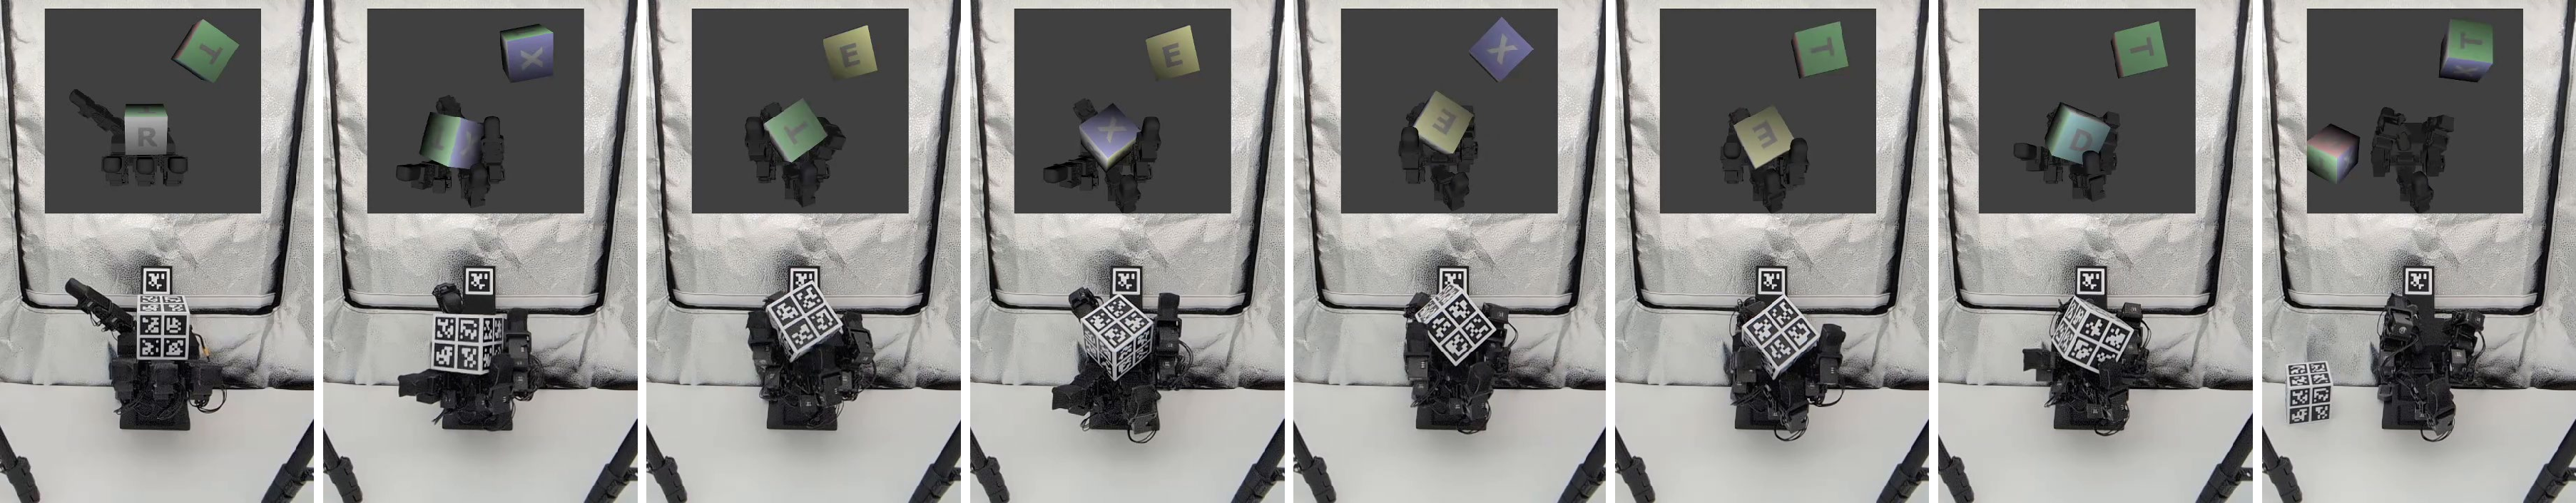
\includegraphics[width=\linewidth]{figures/real_world_results.pdf}
\caption{An example of a real-world run of our policy for in-hand cube reorientation.}
\label{fig:real_world_example}
\vspace{-2mm}
\end{figure}

We deploy our method on a physical LEAP Hand~\cite{shaw2023leaphand} along with a cube pose estimator based on AprilTags~\cite{apriltag,park2026aprilcube} (Fig.~\ref{fig:real_world_example}). Details of our cube pose estimation algorithm are presented in Appendix~\ref{appendix:cube_pose}. To reduce the sim-to-real gap, we performed system identification on the entire hardware setup with details provided in Appendix~\ref{appendix:sys_ID}. We evaluate in-hand cube reorientation over 10 independent trials per method. In each trial, the policy runs continuously until the cube falls off the hand. Table~\ref{tab:real_world} reports the number of consecutive successful reorientations achieved before failure in each trial, along with the mean across trials. 

We observe a significant performance gap between simulation and the real world despite our efforts on system identification and domain randomization. However, all variants of our method outperform the joint-control baseline. Notably, even the zero-shot UHAS model achieved higher average consecutive reorientations than the baseline. We further observe that the model trained exclusively on the LEAP Hand achieves the best real-world performance (mean of 2.0). Interestingly, the model trained on multiple hands underperforms the single-hand LEAP model. We attribute this to the fact that single-hand training allows the policy to exploit the specific workspace and kinematics of the LEAP Hand, whereas multi-hand training forces the network to learn only movements that are feasible and safe across all hands. Given the relatively simple actor-critic architecture, this results in a more conservative policy when trained on multiple embodiments. Please see the supplementary video for the real-world deployment, and additional results in Appendix~\ref{appendix:results}.

% To facilitate object pose tracking, we utilize custom 3D printed AprilTag markers built into the cube based on a modified aprilcube design. (cite) Previous attempts with printed stickers attached to the cube proved to be too fragile for constant contact with the hand. A RealSense D435 camera mounted on a static tripod tracks these markers alongside a reference AprilTag affixed to the leap hand's base. By computing transformations between the camera, the base, and the object, we map the cube's pose from the camera coordinate frame into the sphere frame for the model observations.




% \begin{table}[h!]
%     \centering
%     \caption{Real-world cube reposing on the LEAP Hand (10 independent trials).}
%     \label{tab:real_world}
%     \begin{tabular}{lcc}
%         \toprule
%         \textbf{Method} & \textbf{Mean Successful Reposes} & \textbf{Success Rate (\%)} \\
%         \midrule
%         UGAS (Trained on LEAP only)     & 5.90 & 83.96 \\
%         UGAS (LEAP OOD)     & 2.0 & 66.66 \\
%         % UGAS (Trained on All Grippers)  & 1.6 & 61.54 \\ 
%         UGAS (Trained on All Grippers)  & 2.8 & 73.68 \\ 
%         Baseline (Isaac Sim Joints)     & 0.70 & 41.18  \\
%         \bottomrule
%     \end{tabular}
% \end{table}




